\section{Methodology}
\label{sec:methodology}
% Focus on what you add to the existing method. Explain what you will do and why (and how). Do not forget to characterize your research design. There should be an evaluation plan in this section. (For DS students, this normally means using manually labelled or ground truth data.)

\todo[inline]{Very much still a work in progress}

% ============================================================================ %
% Description of the data
% ============================================================================ %
\subsection{Description of the data}

The data used in this study was simulated using the open-source Bilby code~\cite{Ashton_Bilby_2019}. The gravitational waveforms of three LIGO detectors (Hanford, Washington and Livingston) were generated as a function of 15 independent parameters. Ten of these parameters represented intrinsic properties of the source e.g. the masses and spins of the two black holes, while five of these are extrinsic parameters e.g. the distance from the source and orientation in the sky with respect to the observations. Further details of the parameters are listed in Table~\ref{tab:gw_parameters}. Simulating the waveforms for training the neural network is necessary since we need $\sim$100000 waveforms for training and experimentally measured signals are rare (only 90 detections so far).

Only low SNR case considered because high SNR is unrealistic and it is important for the network to determine signal from noise.

\todo[inline]{Complete table}

\begin{table}[htb]
\centering
\begin{tabular}{|l|l|l|l|}
\hline
\textbf{Parameter} & \textbf{Type} & \textbf{Prior} & \textbf{Test Value} \\
\hline
Mass ratio, \( q \) & I & \( U(0.125, 1) \) & 0.8858 \\
Chirp mass \( M \) [\( M_{\odot} \)] & I & \( U(25, 100) \) & 32.14 \\
Inclination angle \( \theta_{jn} \) [rad] & I & sine(0, \( \pi \)) & 0.4432 \\
Phase \( \phi_c \) [rad] & I & \( U(0, 2\pi) \) & 5.089 \\
Tilt angle \( \theta_1 \) [rad] & I & sine(0, \( \pi \)) & 1.497 \\
Tilt angle \( \theta_2 \) [rad] & I & sine(0, \( \pi \)) & 1.102 \\
Spin \( a_1 \) & I & \( U(0.05, 1) \) & 0.9702 \\
Spin \( a_2 \) & I & \( U(0.05, 1) \) & 0.8118 \\
Spin angle \( \phi_{12} \) [rad] & I & \( U(0, 2\pi) \) & 6.220 \\
Spin angle \( \phi_{jl} \) [rad] & I & \( U(0, 2\pi) \) & 1.885 \\
Luminosity Distance \( d_L \) [Mpc] & E & \( U_{\text{vol}}(100, 2000) \) & 900 \\
Right ascension \( \alpha \) [rad] & E & \( U(0, 2\pi) \) & 5.556 \\
Declination \( \delta \) [rad] & E & cosine(-\( \pi/2 \), \( \pi/2 \)) & 0.071 \\
Polarisation angle \( \psi \) [rad] & E & \( U(0, \pi) \) & 1.100 \\
Merger time \( t_c \) [GPS s] & E & \( U(-0.1, 0.1) \) & 0.000 \\
\hline
\end{tabular}
\caption{Description and type of the parameters that fully describe the detected gravitational waves.}
\label{tab:gw_parameters}
\end{table}

The waveform data consists of 1D signals in both time and frequency domains, collected from the three separate detectors that have captured the event simultaneously. An example of the signal in the time domain is shown in Figure~\ref{fig:obs_time_domain}. In total, there are 8192 channels corresponding to 4\,s of collection time at a sampling frequency of 2048\,Hz. With the Fourier transform, the time signal is decomposed into its constituent frequency components. Both the time and frequency domains are fed into the neural network, since they have different information about the parameters encoded. An example of the signal in the frequency domain is shown in Figure~\ref{fig:obs_freq_domain}.

\begin{figure}
  \centering
  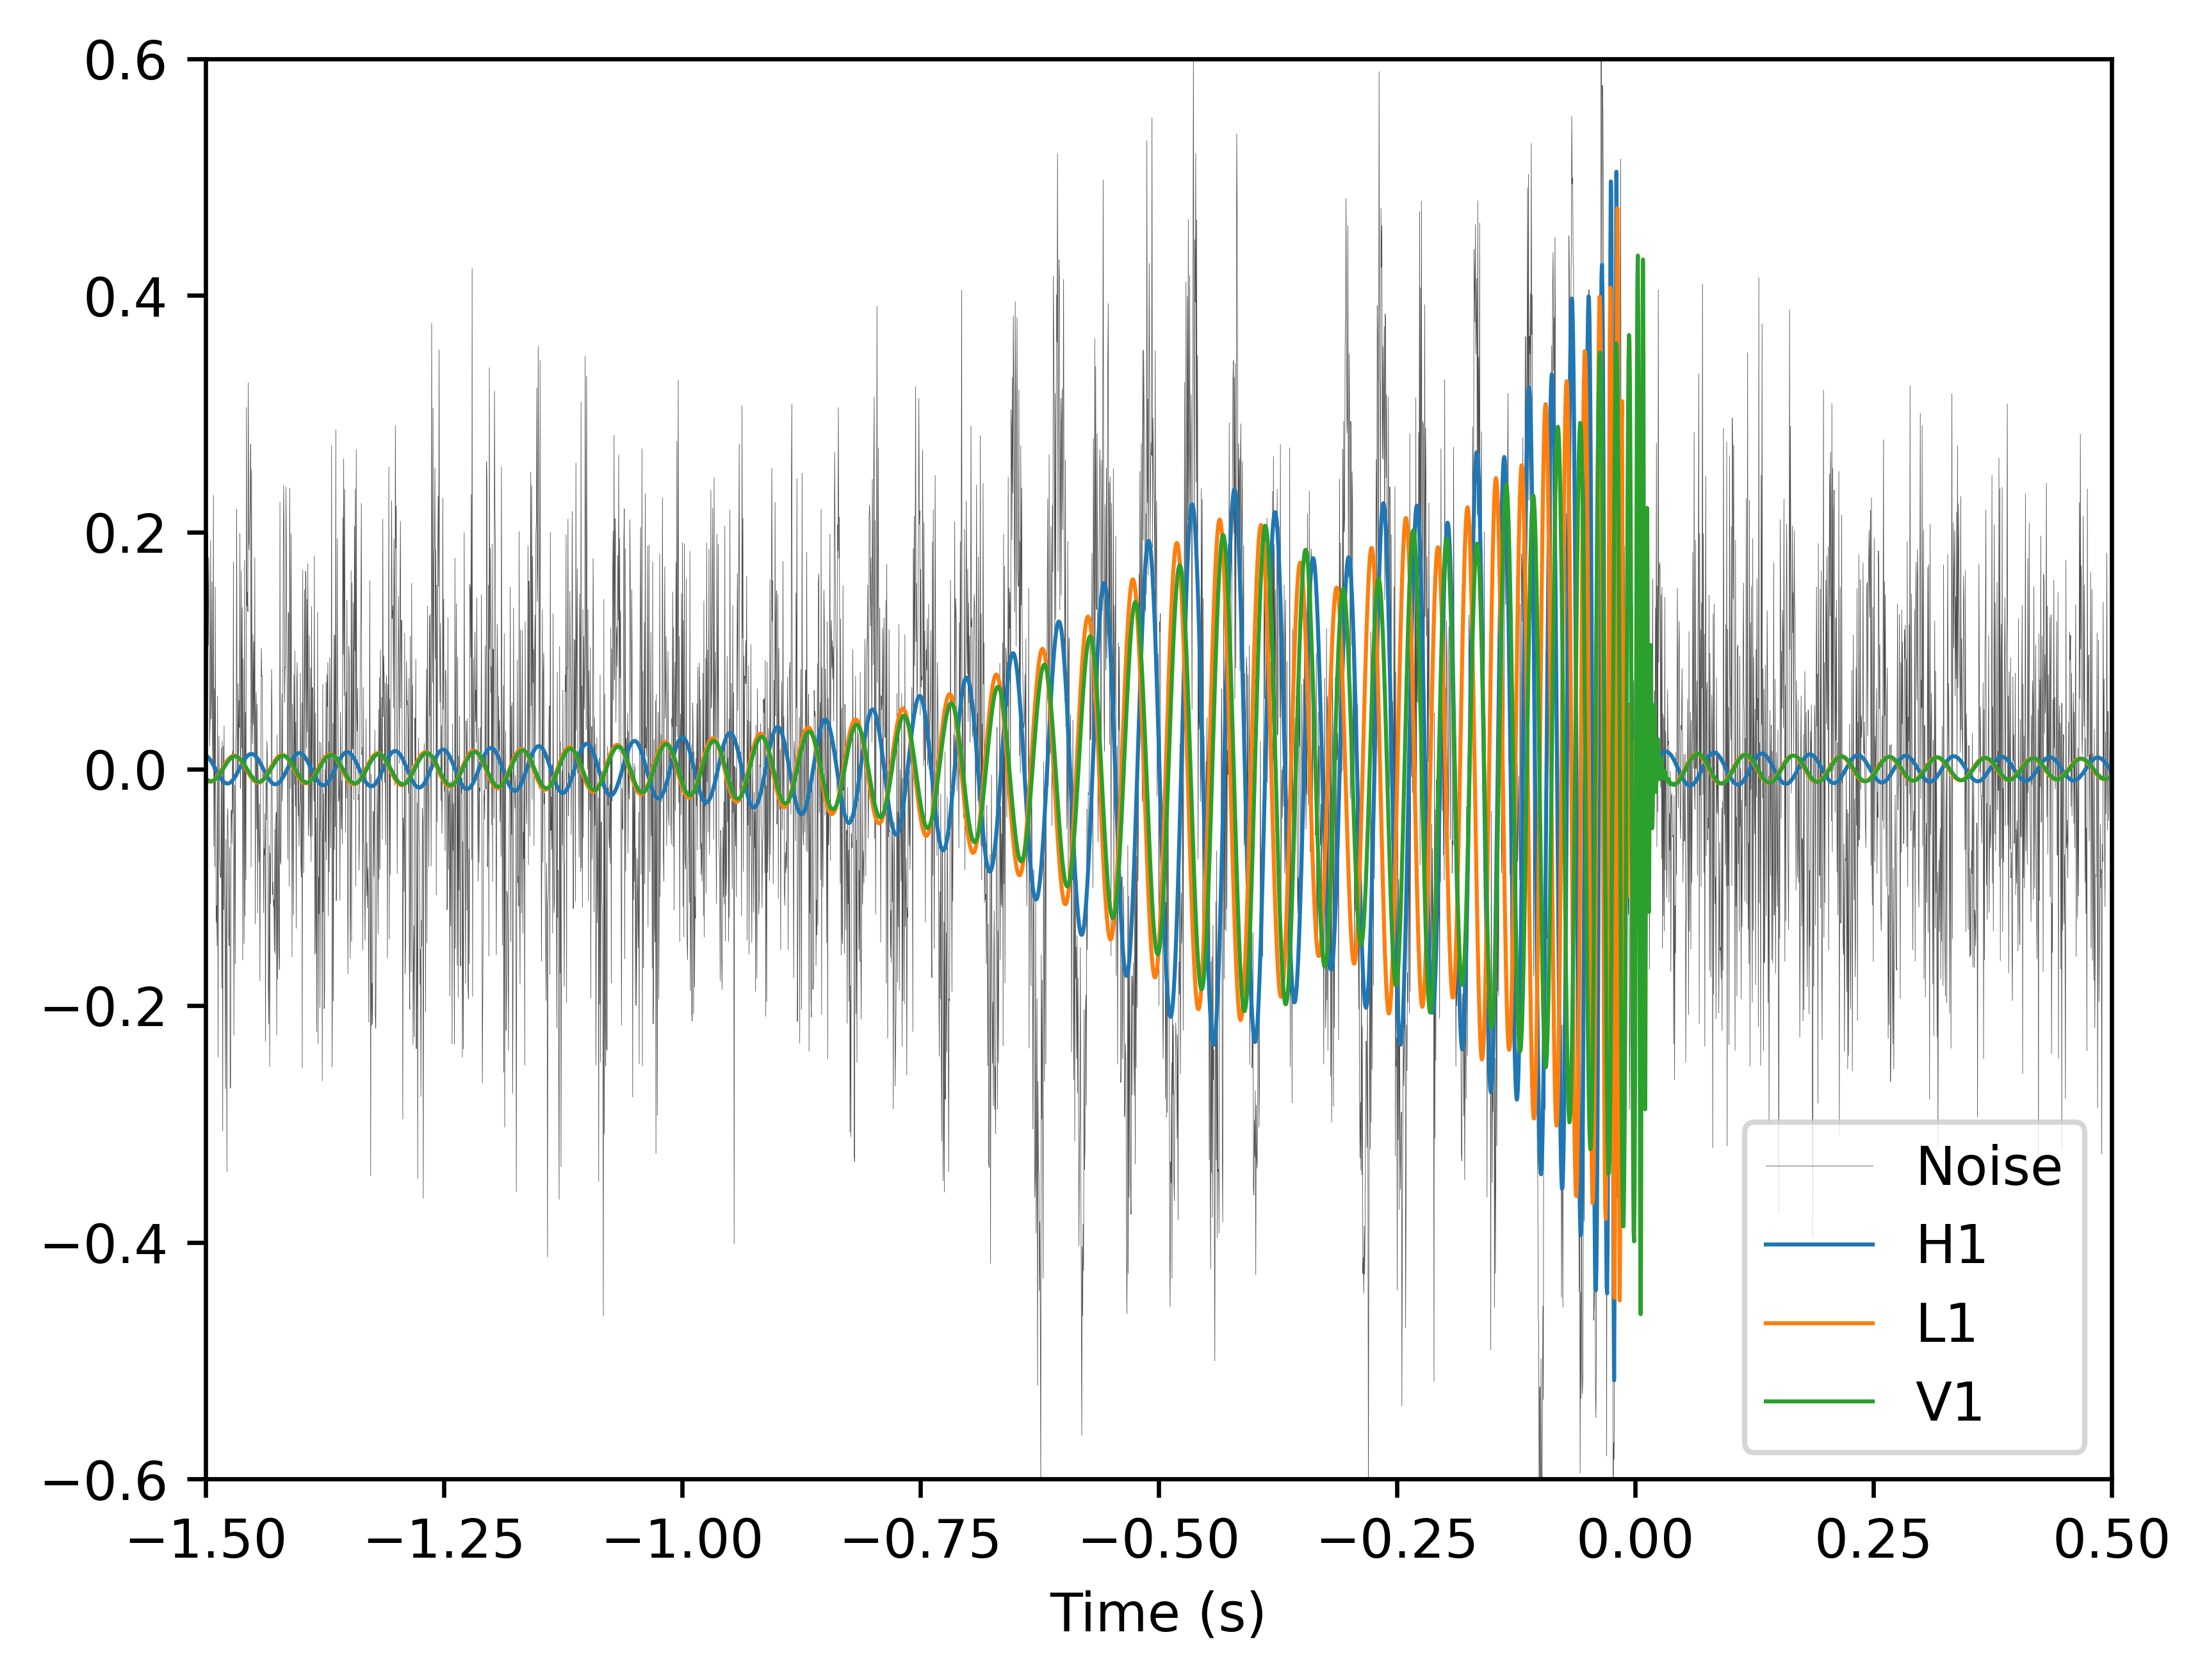
\includegraphics[width=1\linewidth]{media/images/obs_time_domain_lowSNR.png}
  \caption{Example of generated gravitational wave signal in the time domain. Signals from three detectors are shown. For clarity, the noise and signal are shown separately in the figure, but are added together when training the network. The two black holes merge at the moment t=0s. }
  \label{fig:obs_time_domain}
\end{figure}

\begin{figure}
  \centering
  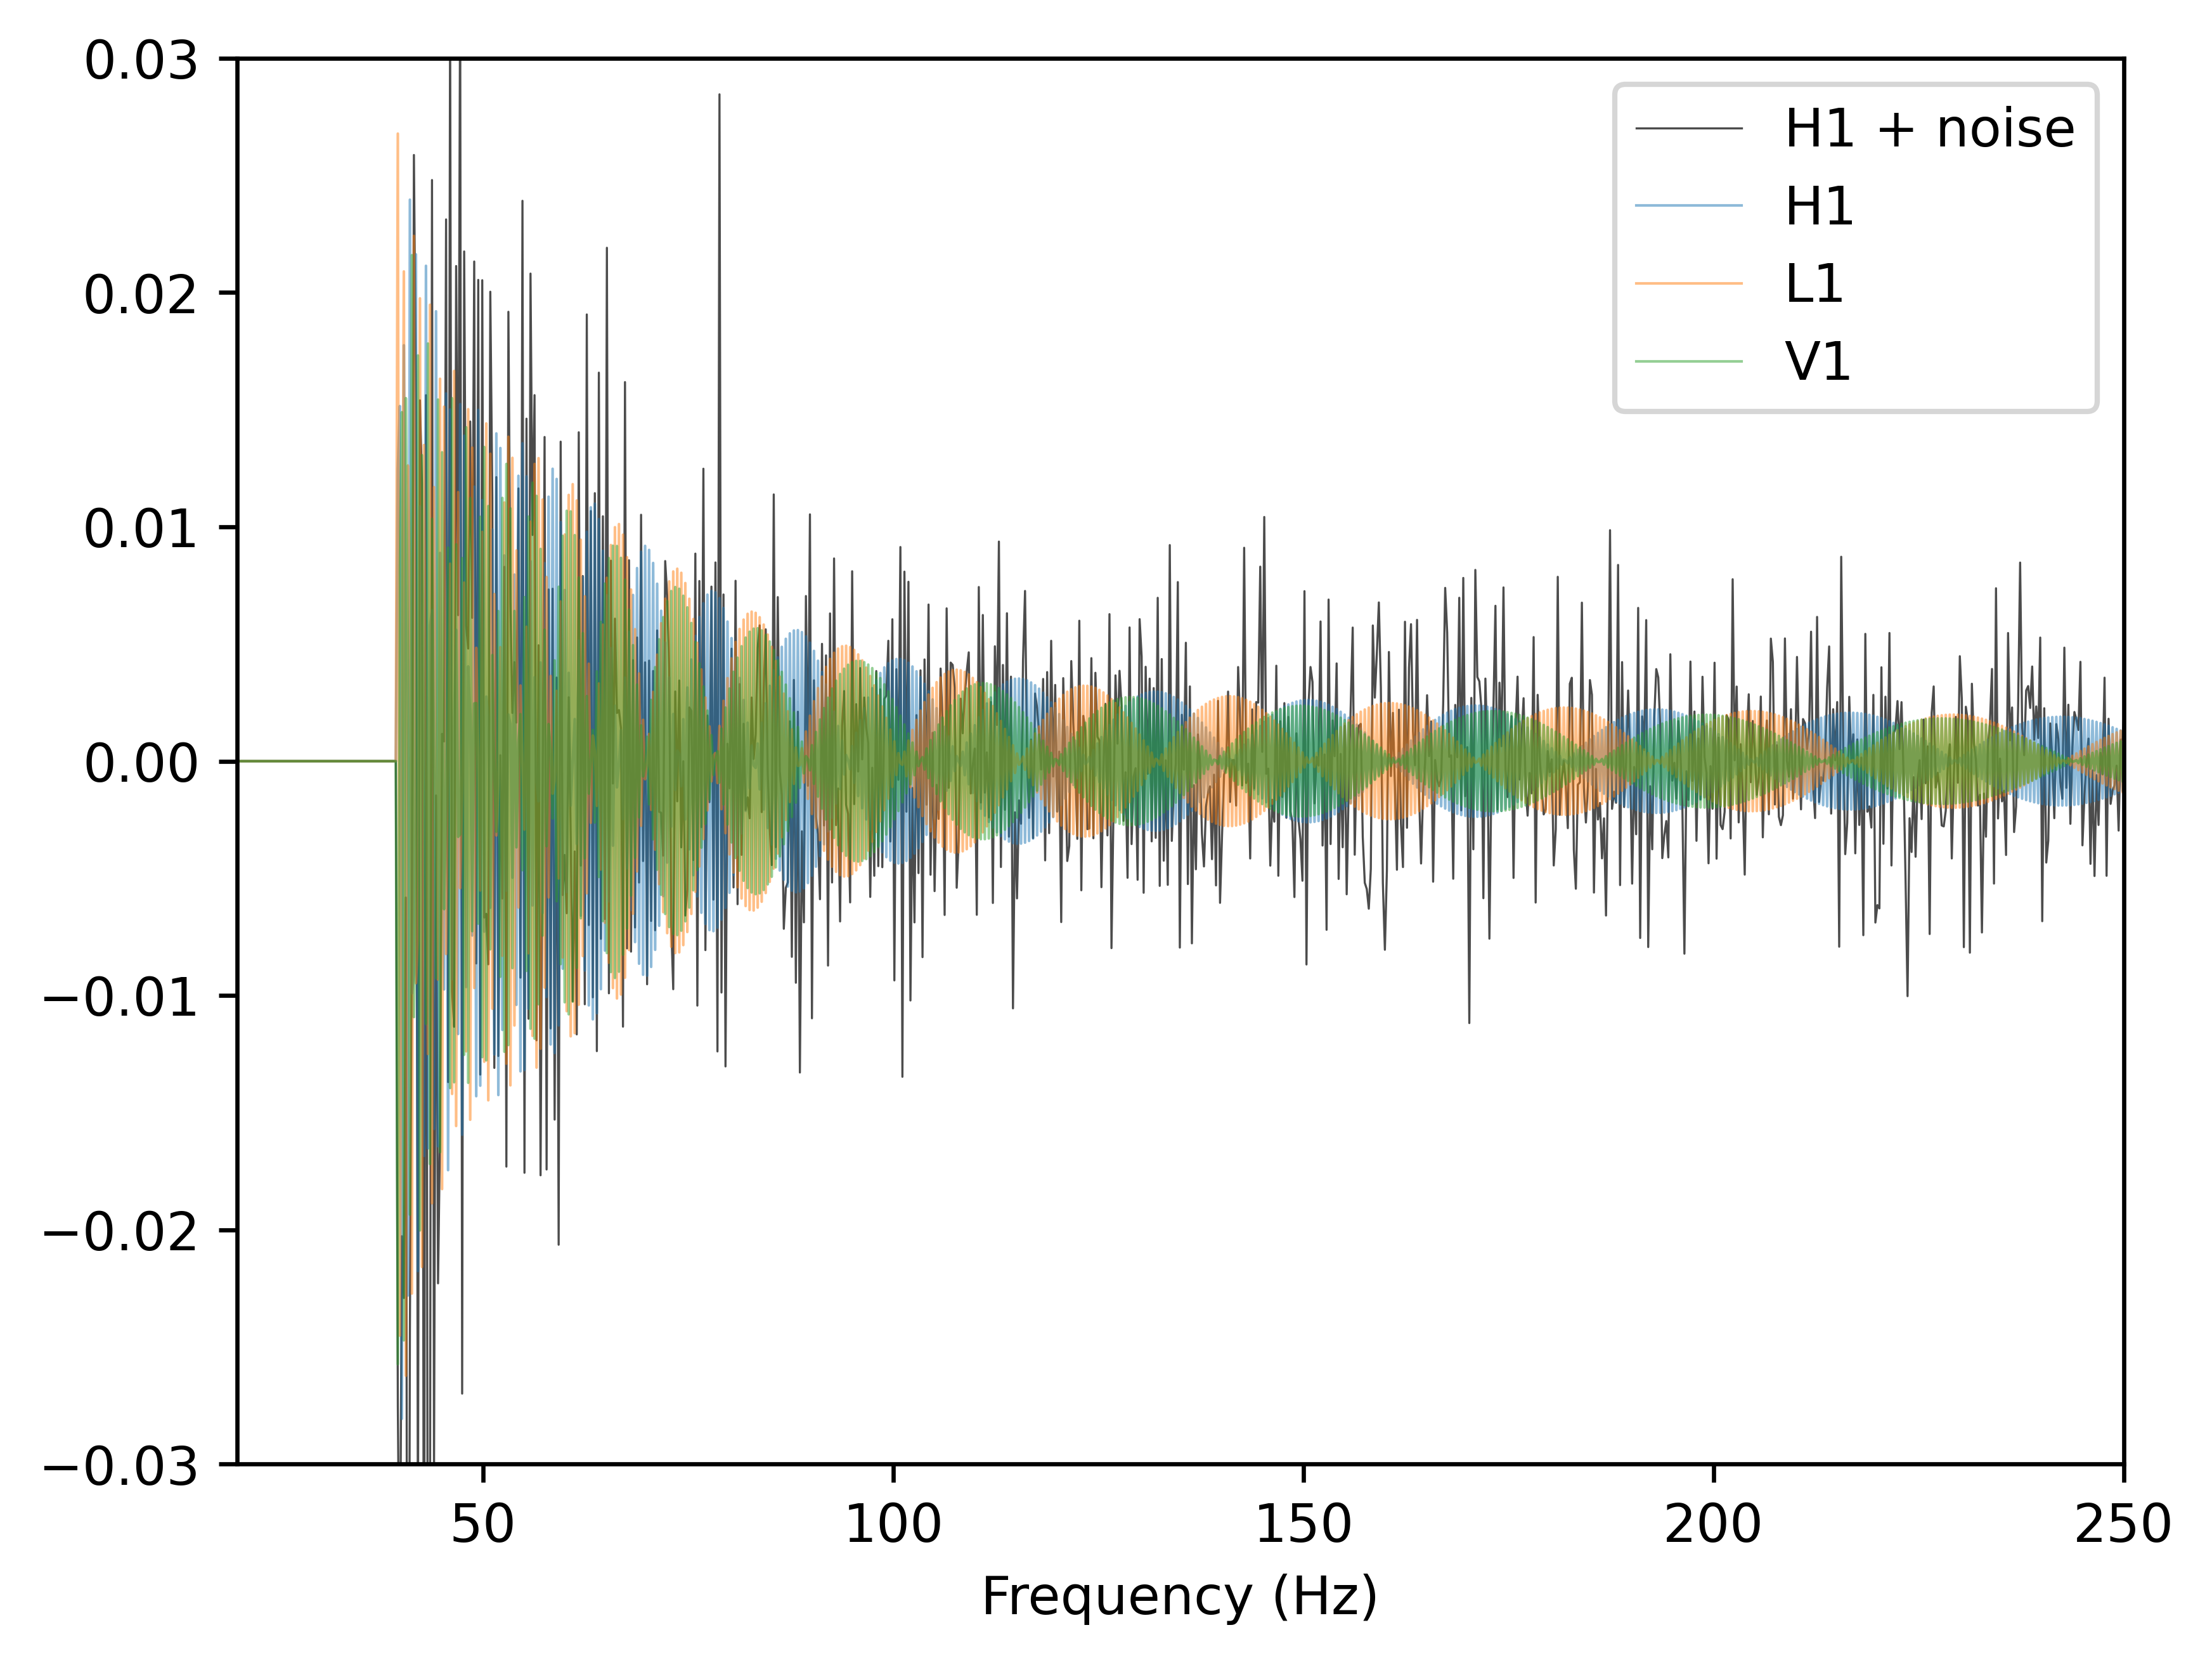
\includegraphics[width=1\linewidth]{media/images/obs_freq_domain_lowSNR.png}
  \caption{Example of generated gravitational wave signal in the frequency domain. Signals from three detectors are shown. For clarity, the noise and signal are shown separately in the figure, but are added together when training the network.}
  \label{fig:obs_freq_domain}
\end{figure}

Only low signal to noise signal will be considered here since the high SNR is unphysical and the low SNR is more challenging. Many moving parts to problem - number of truncation rounds, the number of simulations per round, network architecture, the truncation, the sampling strategy of the priors.

% ============================================================================ %
% Peregrine
% ============================================================================ %
\subsection{Peregrine inference pipeline}

The overall objective of this work is to increase the efficiency of the \texttt{Peregrine} data analysis pipeline. The work will begin with reproducing the results from papers~\cite{bhardwaj2023peregrine} and~\cite{alvey2023things}, as this will form the benchmark to which the eventual results will be compared to.

The workflow for the simulation-based inference technique for the analysis of the gravitational wave signals as implemented in \texttt{peregrine}~\cite{bhardwaj2023peregrine} is shown in Figure~\ref{fig:peregrine_pipeline}. The process starts by setting the 15 parameters of the `target observation' and then generating the example waveform to be analysed. This is done so there are `ground-truth' parameter values that you can compare your final posterior probability density distributions with and validate the overall method. If we use a true experimentally measured signal, then we can never know for certain what the `ground-truth' values of the parameters are. Given the accuracy that we can forward model the GW signals with, once the method is validated with the simulated waveforms, it is expected to work equally well with true experimental measurements.

\begin{figure}[htb]
    \centering
    \begin{tikzpicture}[node distance=2cm]
        \node (sampling) [sample] {\textbf{Sample} parameters $\boldsymbol{\theta}_{GW}$ from prior $p(\boldsymbol{\theta}_{GW})$};
        \node (fsimulator) [simulator, below of=sampling] {\textbf{Simulate} data $\boldsymbol{x}(\theta_{GW}) = h(\theta_{GW}) + n_{IFO}$};
        \node (network) [network, below of=fsimulator, yshift=-0.25cm] {\textbf{Train} CNN to estimate likelihood-to-evidence ratios $r(\boldsymbol{x};\theta_k) = p(\theta_k|\boldsymbol{x})/p(\theta_k)$ for all parameters $k$};
        \node (inference) [inference, below of=network] {Bayesian \textbf{Inference}};
        \node (prior) [pinput, left of=inference, xshift=-1cm] {Prior sample from $p(\theta)$};
        \node (target) [tinput, right of=inference, xshift=1cm] {Target Observation $\boldsymbol{x}_0$};
        \node (ratios) [output, below of=inference, xshift=-1.5cm] {Ratios $r(\boldsymbol{x}_0;\theta)$};
        \node (posterior) [output, below of=inference, xshift=1.5cm] {Posteriors $p(\theta|\boldsymbol{x}_0)$};
        \draw [arrow] (sampling) -- node[anchor=west] {$\boldsymbol{\theta}_{GW}$} (fsimulator);
        \draw [arrow] (fsimulator) -- node[anchor=west] {$\boldsymbol{\theta}_{GW},\boldsymbol{x}$} (network);
        \draw [arrow] (network) -- (inference);
        \draw [arrow] (prior) -- (inference);
        \draw [arrow] (target) -- (inference);
        \draw [arrow] (inference) -- (posterior);
        \draw [arrow] (inference) -- (ratios);
        \draw [arrow] (ratios) -- +(-3,0) |- node[anchor=west, yshift=-2cm, text width=2cm]{Using $r(\boldsymbol{x}_0;\theta)$ update prior $p(\boldsymbol{\theta}_{GW})$ and repeat rounds until converged} (sampling);
    \end{tikzpicture}
    \caption{High-level overview of the simulation-based inference method used for this work.}
    \label{fig:peregrine_pipeline}
\end{figure}


Fifteen individual binary classifiers. Minimise binary cross-entropy loss.

Noise shuffling.

% \subsection{Optimising of sampling efficiency}

% We will investigate whether some more active learning can be introduced to increase the efficiency of the sampling process. For instance, some parameters such as the chirp mass\footnote{The chirp mass is a combination of the two object masses in the binary system, and is a key factor in the gravitational wave frequency as the two objects spiral inwards toward each other.\\$\mathcal{M} = \frac{(m_1 \cdot m_2)^{3/5}}{(m_1 + m_2)^{1/5}}$} may be inferred early on with relatively high confidence, but currently in successive simulation rounds continues to be sampled from a uniform distribution within $\pm5\sigma$~\cite{Miller_TMNRE_2021}. We will investigate whether it's possible to be more selective in the sampling of parameters that are known with relatively high confidence in an un-biased way. Therefore, we can focus the simulation budget more on the parameters we know with less confidence. To do this in a systematic way, a complete survey of how influential each parameter is on the different segments of the GW signal will be carried-out first.

The current rendition of the Peregrine pipeline requires 8 rounds of sequential TMNRE, 720000 simulated waveforms and around 12.5 hours (on a single A100 gpu with 18 cpu cores) to completely reconstruct the posteriors of the fifteen parameters. Of these 12.5 hours, around 10 is for training the network and 2.3 is for generating the waveforms used for training the network. Our primary focus is therefore the optimisation of the pipeline on the network itself, and as a secondary the number of simulated waveforms.

Trainer settings.

% ============================================================================ %
% Overview
% ============================================================================ %
\subsection{Overview of approach}

Focus on the loss 

% ============================================================================ %
% Transformer models
% ============================================================================ %
\subsection{Transformer models}



\subsubsection{Hyperparameter tuning}

RayTune was used to tune hyperparameters. 

\subsubsection{Pretraining}

Transformers were pretrained for 24 hours with single A100 gpu on 2 million waveforms.


% ============================================================================ %
% Attention U-Net
% ============================================================================ %
\subsection{Attention U-Net}



% ============================================================================ %
% Pruning
% ============================================================================ %
\subsection{Pruning}


%The architecture of the network currently implemented in \texttt{peregrine} is the U-Net architecture~\cite{Ronneberger_UNet_2015}. Given the advances in machine learning and CNN architectures since 2015, it is believed that this network can be improved upon. The optimisation of this network architecture will be the main focus of this thesis. 

%Investigative studies will be performed to find the best network architectures most suitable for the data format. We will first try with LSTM's since they are known to work well with noisy time-series data. The chosen network architecture also needs to be capable of segmenting the signal into three components, representing the different stages of the merger event -- inspiral, merger and ringdown~\cite{Pan_GW_2014}. Each of the parameters in $\boldsymbol{\theta}_{GW}$ are impacted differently in the different phases~\cite{bhardwaj2023peregrine}. Given the network is a binary classifier that classifies between joint and marginally drawn sample pairs, we will assess the performance of the network with the ROC curve.


% ============================================================================ %
% Evaluation
% ============================================================================ %
\subsection{Evaluation}

%The changes to the \texttt{peregrine} analysis pipeline will be fully benchmarked against the original \texttt{peregrine}, both in terms of accuracy of final result and required runtime. The results of the original \texttt{peregrine} have themselves been benchmarked against established likelihood-based methods~\cite{Speagle_2020}, and found to be in good agreement. Therefore, in this work we think it is sufficient to compare only with the original \texttt{peregrine}. To demonstrate the applicability of the method to real gravitational wave measurements, if time permits, we will also test the approach using real experimental data.

